% !TeX root = chapter-4-5.tex

\chapter{טריגונומטריה}

\begin{comment}

\section{קיץ תשע"ח מועד ב}

\begin{center}
\selectlanguage{english}
\includegraphics[width=\textwidth]{summer-2018b-5}
\end{center}

%%%%%%%%%%%%%%%%%%%%%%%%%%%%%%%%%%%%%%%%%%%%%%%%%%%%%%%%%%%%%%
\np

\section{קיץ תשע"ח מועד א}

\begin{center}
\selectlanguage{english}
\includegraphics[width=\textwidth]{summer-2018a-5}
\end{center}

%%%%%%%%%%%%%%%%%%%%%%%%%%%%%%%%%%%%%%%%%%%%%%%%%%%%%%%%%%%%%%
\np

\section{חורף תשע"ח}

\begin{center}
\selectlanguage{english}
\includegraphics[width=\textwidth]{winter-2018-5}
\end{center}

%%%%%%%%%%%%%%%%%%%%%%%%%%%%%%%%%%%%%%%%%%%%%%%%%%%%%%%%%%%%%%
\np

\section{קיץ תשע"ז מועד ב}

\begin{center}
\selectlanguage{english}
\includegraphics[width=\textwidth]{summer-2017b-5}
\end{center}

%%%%%%%%%%%%%%%%%%%%%%%%%%%%%%%%%%%%%%%%%%%%%%%%%%%%%%%%%%%%%%
\np

\end{comment}

\section{קיץ תשע"ז מועד א}

\begin{center}
\selectlanguage{english}
\includegraphics[width=\textwidth]{summer-2017a-5}
\end{center}

\textbf{סעיף א}

הופסנו סימונים תוך הסתמכות על הנתון ש-%
$\triangle ABC$
שווה שוקיים,
$AF,BD,CF$
תיכונים, ומשפט

$46$
"נקודת חיתוך התיכונים מחלקת כל תיכון ביחס 
$2:1$".
כמו כן,
$AF=CE$
כי
$\triangle AEC\cong \triangle CEA$
לפי צ.ז.צ.

\begin{center}
\selectlanguage{english}
\begin{tikzpicture}[scale=1.1]
\draw[thick] (0,0) coordinate (A) node[left] {$A$} -- (8,0) coordinate (C) node[right] {$C$} -- (4,4.5) coordinate (B) node[above] {$B$} -- cycle;
\fill (A) circle(1.5pt);
\fill (B) circle(1.5pt);
\fill (C) circle(1.5pt);
\coordinate (D) at ($(A)!.5!(C)$);
\coordinate (E) at ($(A)!.5!(B)$);
\coordinate (F) at ($(C)!.5!(B)$);
\fill (D) node[below] {$D$} circle(1.5pt);
\fill (E) node[left,xshift=-2pt,yshift=2pt]  {$E$} circle(1.5pt);
\fill (F) node[right,xshift=2pt,yshift=2pt] {$F$} circle(1.5pt);
\draw (D) rectangle +(8pt,8pt);
\draw[thick,name path=af] (A) -- (F);
\draw[thick,name path=ce] (C) -- (E);
\draw[thick,name path=bd] (B) -- (D);
\path[name intersections={of=af and ce,by={O}}];
\fill (O) node[above right,yshift=2pt] {$O$} circle(1.5pt);
\path (A) -- node[below] {$a/2$} (D) -- node[below] {$a/2$} (C);
\path (A) -- node[left] {$b/2$} (E) -- node[left] {$b/2$} (B);
\path (C) -- node[right] {$b/2$} (F) -- node[right] {$b/2$} (B);
\path (B) -- node[right] {$2r$} (O) -- node[right] {$r$} (D);
\path (A) -- node[above] {$2c$} (O) -- node[below] {$c$} (F);
\path (C) -- node[above] {$2c$} (O) -- node[below] {$c$} (E);
\draw[thick,dashed,name path=ef] (E) -- (F);
\path[name intersections={of=ef and bd,by={G}}];
\fill (G) node[above left] {$G$} circle(1.5pt);
\draw (G) rectangle +(8pt,8pt);
\end{tikzpicture}
\end{center}

נשתמש במשפט
$91$
"משפט תאלס המורחב: ישר המקביל לאחת מצלעות המשולש חותך את שתי הצלעות האחרות או את המשכיהן בקטעים פרופורציוניים", כך ש-%
$EF=\displaystyle\frac{AC}{2}=\frac{a}{2}$:
\erh{14pt}
\begin{equationarray*}{rcl}
S_{BOE}&=&\frac{1}{2}\cdot \frac{a}{4}\cdot BG+\frac{1}{2}\cdot \frac{a}{4}\cdot GO\\
&=&\frac{1}{2}\cdot \frac{a}{4}\cdot 2r\\
&=&\frac{1}{4}ar\\
S_{COD} &=& \frac{1}{2}r\cdot \frac{a}{2}\\
&=&=\frac{1}{4}ar\,.
\end{equationarray*}

%%%%%%%%%%%%%%%%%%%%%%%%%%%%%%%%%%%%%%%%%%%%%%%%%%%%%%%%%%%%%%

\begin{comment}
\np

\section{חורף תשע"ז}

\begin{center}
\selectlanguage{english}
\includegraphics[width=\textwidth]{winter-2017-5}
\end{center}


%%%%%%%%%%%%%%%%%%%%%%%%%%%%%%%%%%%%%%%%%%%%%%%%%%%%%%%%%%%%%%
\np

\section{קיץ תשע"ו מועד ב}

\begin{center}
\selectlanguage{english}
\includegraphics[width=\textwidth]{summer-2016b-5}
\end{center}

%%%%%%%%%%%%%%%%%%%%%%%%%%%%%%%%%%%%%%%%%%%%%%%%%%%%%%%%%%%%%%
\np

\section{קיץ תשע"ו מועד א}

\begin{center}
\selectlanguage{english}
\includegraphics[width=\textwidth]{summer-2016a-5}
\end{center}

%%%%%%%%%%%%%%%%%%%%%%%%%%%%%%%%%%%%%%%%%%%%%%%%%%%%%%%%%%%%%%
\np

\section{חורף תשע"ו}

\begin{center}
\selectlanguage{english}
\includegraphics[width=\textwidth]{winter-2016-5}
\end{center}

%%%%%%%%%%%%%%%%%%%%%%%%%%%%%%%%%%%%%%%%%%%%%%%%%%%%%%%%%%%%%%
\np


\section{קיץ תשע"ה מועד ב}

\begin{center}
\selectlanguage{english}
\includegraphics[width=\textwidth]{summer-2015b-5}
\end{center}

\vspace{-1ex}

\textbf{סעיף א}

הוספנו סימונים לתרשים ונצטרך להצדיק אותם. 
משפט
$77$
"המשיק למעגל מאונך לרדיוס בנקודת ההשקה" ולכן הקו 
$EF$
הניצב לצלעות המקיבלים 
$AB\|DC$
הוא באורך
$2r$.
$AG, BH$
אנכים מ-%
$AB$ 
ל-%
$DC$,
כך ש-%
$AG=EF=BF=2r$,
ו-%
$AB=GH=b_2$.
הטרפז שווה-שוקיים ולפי משפט
$39$
"בטרפז שווה שוקיים הזוויות שליד אותו בסיס שוות זו לזו", 
$\angle ADC=\angle BCD=70^\circ$.

\begin{center}
\selectlanguage{english}
\begin{tikzpicture}[scale=1.1]
\node[circle,draw,thick] (In) at (0,0) [minimum size=5.45cm] {};
\fill (In) circle(1.5pt);
\coordinate (D) at (-3.5,-2.5);
\draw[thick] (D) -- +(7,0) coordinate (C) node[above left,xshift=-2pt] {$70$};
\fill (C) node[below right] {$C$} circle(1.5pt);
\fill (D) node[below left] {$D$}  node[above right,xshift=2pt] {$70$} circle(1.5pt);
\coordinate (DA) at (tangent cs:node=In,point={(D)},solution=2);
\path[name path=da] (D) -- ($(D)!1.7!(DA)$);
\fill (DA) circle(1.5pt);
\coordinate (CB) at (tangent cs:node=In,point={(C)},solution=1);
\path[name path=cb] (C) -- ($(C)!1.7!(CB)$);
\fill (CB) circle(1.5pt);
\path[name path=top] (-3,2.5) -- (3,2.5);
\path[name intersections={of=da and top,by={A}}];
\path[name intersections={of=cb and top,by={B}}];
\fill (A) node[above left] {$A$} circle(1.5pt);
\fill (B) node[above right] {$B$} circle(1.5pt);
\draw[thick] (D) -- node[left] {$s$} (A) -- (B) -- node[right] {$s$} (C);
\draw[thick,dashed] (D) -- (B);
\coordinate (AB) at (0,2.5);
\fill (AB)  node[above] {$E$} circle (1.5pt);
\coordinate (DC) at (0,-2.5);
\fill (DC)  node[below,yshift=-1pt] {$F$} circle (1.5pt);
\draw[thick,dashed] (AB) -- node[left,yshift=-6pt] {$2r$} (DC);
\coordinate (ADC) at ($(D)!(A)!(C)$);
\draw[thick,dashed] (A) -- node[right,yshift=8pt] {$2r$} (ADC);
\fill (ADC) node[below,yshift=-1pt] {$G$} circle(1.5pt);
\coordinate (BDC) at ($(D)!(B)!(C)$);
\draw[thick,dashed] (B) -- node[left,yshift=8pt] {$2r$} (BDC);
\fill (BDC) node[below,yshift=-1pt] {$H$} circle(1.5pt);
\draw (ADC) rectangle +(8pt,8pt);
\draw (BDC) rectangle +(8pt,8pt);
\draw (DC) rectangle +(8pt,8pt);
\draw[<->] ($(D)+(0,-8mm)$) -- node[fill=white] {$b_1$} ($(ADC)+(0,-8mm)$);
\draw[<->] ($(ADC)+(0,-8mm)$) -- node[fill=white] {$b_2$} ($(BDC)+(0,-8mm)$);
\draw[<->] ($(BDC)+(0,-8mm)$) -- node[fill=white] {$b_1$} ($(C)+(0,-8mm)$);
\draw[<->] ($(D)+(0,-14mm)$) -- node[fill=white] {$b$} ($(C)+(0,-14mm)$);
\draw[<->] ($(A)+(0,8mm)$) -- node[fill=white] {$b_2$} ($(B)+(0,8mm)$);
\end{tikzpicture}
\end{center}

\np

$\triangle ADG \cong \triangle BCH$
לפי ז.צ.ז: מהשלמת הזוויות במשולשים,
$\angle DAG=\angle CBH=180-90-70$.
מכאן ש-%
$DG=HC=b_1$,
והבסיס הוא
$b=2b_1+b_2$.

כעת נוכל לגשת לחישוב הערכים המבוקשים בסעיף.


$(1)$
לפי משפט
$57$
"מרובע קמור חוסם מעגל אם ורק אם סכום שתי צלעות נגדיות שווה לסכום שתי הצלעות הנגדיות האחרות":
\vspace{-6ex}

\erh{12pt}
\begin{equationarray*}{rcl}
2s&=&b_2+(b_1+b_2+b_1)\\
b_2 &=&s-b_1\\
\tan 70 &=& \frac{2r}{b_1}\\
\sin 70&=&\frac{2r}{s}\\
b&=&2b_1+b_2=2b_1+(s-b_1)=b_1+s\\
&=&2r\left(\frac{1}{\tan 70}+\frac{1}{\sin 70}\right)\\
&=&2.856r\,.
\end{equationarray*}

\vspace{-3ex}

$(2)$
$s=\displaystyle\frac{2r}{\sin 70}=2.128r$.

\medskip

$(3)$
האלכסון הוא היתר של 
$\triangle BDH$
שצלעותיו ידועים:

\vspace{-6ex}

\erh{18pt}
\begin{equationarray*}{rcl}
DB^2&=& (b_1+b_2)^2 + (2r)^2\\
&=&s^2 +(2r)^2\\
&=& \left(\frac{2r}{\sin 70}\right)^2 + 4r^2\\
DB&=&2r\sqrt{\left(\frac{1}{\sin 70}\right)^2+1}\\
&=&2.921r\,.
\end{equationarray*}

\vspace{-3ex}

\textbf{סעיף ב}

במבט ראשון נראה שכדאי להשתמש במשפט
$56$
"ניתן לחסום מרובע במעגל אם ורק אם סכום זוג זוויות נגדיות שווה ל-%
$180^\circ$",
אבל יש לנו כל כך הרבה מידע על הטרפז שאין בו צורך.


\textbf{שימו לב!!}
המרכז של המעגל החוסם
$M_1$
אינו בהכרח המרכז של המעגל החסום
$M_2$.
ניסיתי לחשב את 
$R$
לפי פיתגורס ב-%
$\triangle FM_2C$
אבל זה לא נכון.

\np

\begin{center}
\selectlanguage{english}
\begin{tikzpicture}[scale=1.1]
\node[circle,draw,thick] (In) at (0,0) [minimum size=5.45cm] {};
\fill (In) circle(1.5pt);
\coordinate (D) at (-3.5,-2.5);
\draw[thick] (D) -- +(7,0) coordinate (C) node[above left,xshift=-2pt] {$70$};
\fill (C) node[below right] {$C$} circle(1.5pt);
\fill (D) node[below left] {$D$} circle(1.5pt);
\coordinate (DA) at (tangent cs:node=In,point={(D)},solution=2);
\path[name path=da] (D) -- ($(D)!1.7!(DA)$);
%\fill (DA) circle(1.5pt);
\coordinate (CB) at (tangent cs:node=In,point={(C)},solution=1);
\path[name path=cb] (C) -- ($(C)!1.7!(CB)$);
%\fill (CB) circle(1.5pt);
\path[name path=top] (-3,2.5) -- (3,2.5);
\path[name intersections={of=da and top,by={A}}];
\path[name intersections={of=cb and top,by={B}}];
\fill (A) node[above left] {$A$} circle(1.5pt);
\fill (B) node[above right] {$B$} circle(1.5pt);
\draw[thick] (D) -- (A) -- (B) -- (C);
\draw[ultra thick] (D) -- (B) -- (C) -- cycle;
\coordinate (AB) at (0,2.5);
\coordinate (DC) at (0,-2.5);
\fill (DC)  node[below,yshift=-1pt] {$F$} circle (1.5pt);
\coordinate (ADC) at ($(D)!(A)!(C)$);
%\draw[thick,dashed] (A) -- node[right,yshift=8pt] {$2r$} (ADC);
%\fill (ADC) node[below,yshift=-1pt] {$G$} circle(1.5pt);
\coordinate (BDC) at ($(D)!(B)!(C)$);
\draw[thick,dashed] (B) -- node[left,yshift=8pt] {$2r$} (BDC);
\fill (BDC) node[below,yshift=-1pt] {$H$} circle(1.5pt);
\draw (BDC) rectangle +(8pt,8pt);
\draw[<->] ($(D)+(0,-8mm)$) -- node[fill=white] {$b_1$} ($(ADC)+(0,-8mm)$);
\draw[<->] ($(ADC)+(0,-8mm)$) -- node[fill=white] {$b_2$} ($(BDC)+(0,-8mm)$);
\tkzCircumCenter(B,D,C)\tkzGetPoint{Cir}
\tkzDrawCircle[thick,dotted,name path=circle](Cir,D)
\fill (Cir) node[right,xshift=2pt,yshift=2pt] {$M_{1}$} circle(1.5pt);
\fill (In) node[above]  {$M_{2}$} circle(1.5pt);
\draw[thick,dotted] (Cir) -- (A);
\draw[thick,dotted] (Cir) -- (B);
\draw[thick,dotted] (Cir) -- (C);
\draw[thick,dotted] (Cir) -- (D);
\end{tikzpicture}
\end{center}
במקום זה יש להשתמש בחוק הסינוסים במשולש
$\triangle BCD$ 
)מודגש(:
\erh{16pt}
\begin{equationarray*}{rcl}
2R&=&\frac{DB}{\sin BCD}=\frac{2.921r}{\sin 70}\\
\frac{r}{R}&=&\frac{2\cdot \sin 70}{2.921}\\
&=&6.434\,.
\end{equationarray*}


%%%%%%%%%%%%%%%%%%%%%%%%%%%%%%%%%%%%%%%%%%%%%%%%%%%%%%%%%%%%%%

\np

\section{קיץ תשע"ה מועד א}

\begin{center}
\selectlanguage{english}
\includegraphics[width=\textwidth]{summer-2015a-5}
\end{center}

\vspace{-1ex}

\textbf{סעיף א}

נסמן בתרשים צלעות וזוויות גם לפי זוויות מתחלפות ומתאימות:
\begin{center}
\selectlanguage{english}
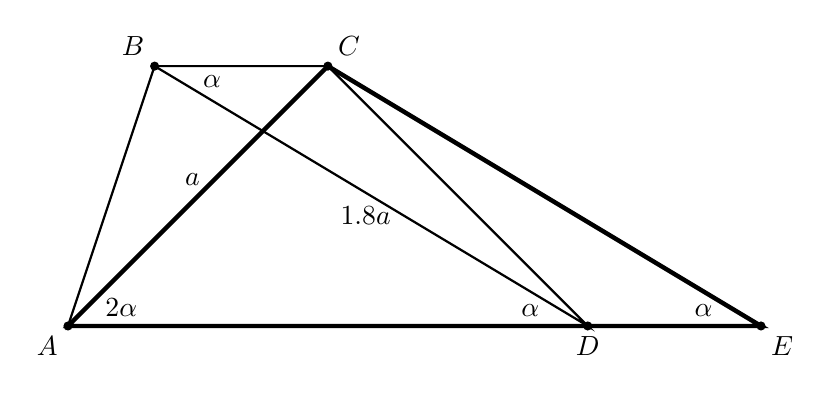
\begin{tikzpicture}[scale=1.1]
\draw[thick] (0,0) coordinate (A) node[below left] {$A$} -- (6,0) coordinate (D) node[below] {$D$} -- (8,0) coordinate (E) node[below right] {$E$} -- (3,3) coordinate (C) node[above right] {$C$} -- (1,3) coordinate (B) node[above left] {$B$} -- (A) -- node[above,xshift=-2pt] {$a$} (C);
\draw[thick] (B) -- node[below,xshift=-2pt] {$1.8a$} (D) -- (C);
\fill (A) node[above right,xshift=10pt] {$2\alpha$} circle(1.5pt);
\fill (B) node[below right,xshift=14pt] {$\alpha$} circle(1.5pt);
\fill (C) circle(1.5pt);
\fill (D) node[above left,xshift=-14pt] {$\alpha$} circle(1.5pt);
\fill (E) node[above left,xshift=-14pt] {$\alpha$} circle(1.5pt);
\draw[ultra thick] (A) -- (E) -- (C) -- cycle;
\end{tikzpicture}
\end{center}

\vspace{-1ex}

כדי לחשב את הזווית 
$\angle CEA=\alpha$
נחפש משלוש שם שני צלעות באורך
$a,1.8a$,
כדי להשתמש בחוק הסינוסים כך שהנעלם
$a$
יצטמצם. אמנם שני הקווים 
$AC,BD$
אינם צלעות של משולש, אבל ניתן לראות ש-%
$BD=CD=1.8a$.
נתון 
$BC\|AD,\,CE\|BD$,
וניתן למשתמש במשפט
$29$
"מרובע שבו כל זוג זוויות נגדיות שוות הוא מקבילית" בגלל זוויות מתחלפות ומתאימות
$\angle CBE,=\angle BDA=\angle CEA=\alpha$,
וזוויות פנימיות
$\angle BCE=\angle BDE=180-\alpha$.

בחוק הסינוסים במשולש המודגש
$ACE$:
\erh{6pt}
\begin{equationarray*}{rcl}
\frac{1}{\sin \alpha} &=& \frac{1.8a}{\sin 2\alpha}\\
1.8\sin \alpha &=& \sin 2\alpha = 2\sin \alpha \cos \alpha\\
\cos \alpha &=& 0.9\\
\alpha &\approx& 25.84\,.
\end{equationarray*}

\np

\textbf{סעיף ב}
נרשום את כל הזוויות במשולש 
$ACE$:
\begin{eqnarray*}
\angle CEA=\alpha &\approx& 25.84\\
\angle CAE=2\alpha &\approx& 51.68\\
\angle ACE=180-3\alpha &\approx& 102.48\,.
\end{eqnarray*}
מהתרשים אפשר לראות ששטח המשולש
$ACE$
מורכב מהשטו של שני משולשים עם אותו גובה:
\begin{center}
\selectlanguage{english}
\begin{tikzpicture}[scale=1.1]
\draw[thick] (0,0) coordinate (A) node[below left] {$A$} -- 
%(6,0) coordinate (D) node[below] {$D$} -- 
(8,0) coordinate (E) node[below right] {$E$} -- (3,3) coordinate (C) node[above right] {$C$} -- (1,3) coordinate (B) node[above left] {$B$} -- (A) -- node[above,xshift=-2pt] {$a$} (C);
%\draw[thick] (B) -- node[below,xshift=-2pt] {$1.8a$} (D) -- (C);
\fill (A) node[above right,xshift=10pt] {$2\alpha$} circle(1.5pt);
\fill (B) circle(1.5pt);
%\fill (B) node[below right,xshift=14pt] {$\alpha$} circle(1.5pt);
\fill (C) circle(1.5pt);
%\fill (D) circle(1.5pt);
%\fill (D) node[above left,xshift=-14pt] {$\alpha$} circle(1.5pt);
\fill (E) node[above left,xshift=-14pt] {$\alpha$} circle(1.5pt);
\draw[ultra thick] (A) -- (E) -- node[right,xshift=2pt,yshift=2pt] {$1.8a$} (C) -- cycle;
\coordinate (F) at ($(A)!(C)!(E)$);
\draw[thick,dashed] (C) -- node[left] {$h$} (F);%($(A)!(C)!(E)$);
\fill (F) circle(1.5pt);
\draw (F) rectangle +(8pt,8pt);
\path (A) -- node[below] {$b_1$} (F) -- node[below] {$b_2$} (E);
\end{tikzpicture}
\end{center}

\vspace{-6ex}

\erh{10pt}
\begin{equationarray*}{rcl}
S_{ACE} &=& \frac{1}{2}(b_1+b_2)h\\
\tan 2\alpha &=& \frac{h}{b_1}\\
\tan \alpha &=& \frac{h}{b_2}\\
S_{ACE} &=& \frac{1}{2}h^2\left(\frac{1}{\tan 2\alpha}+\frac{1}{\tan \alpha}\right)\\
87.873 &=& \frac{1}{2}h^2(6.79+2.06)\\
&=& h^2\cdot 1.425\\
h&\approx& 7.825\,.
\end{equationarray*}
פתרון אחר היא להשתמש בנוסחה לשטח )ששכחתי 
$\ldots$(
שיש לה גורם של סינוס:
\erh{10pt}
\begin{equationarray*}{rcl}
S_{ACE} &=& \frac{1}{2}\cdot AC \cdot CE \cdot \sin ACE\\
&=& \frac{1}{2}\cdot a \cdot 1.8a \cdot \sin (180-3\alpha)\\
87.873 &=& 0.87873 a^2\\
a&=&10\\
h &=& a\sin 2\alpha \approx 7.846\,.
\end{equationarray*}
פתרון זה מעט יותר פשוט ומומלץ למי שלא שכח את הנוסחה.

%%%%%%%%%%%%%%%%%%%%%%%%%%%%%%%%%%%%%%%%%%%%%%%%%%%%%%%%%%%%%%


\np


\section{חורף תשע"ה}

\begin{center}
\selectlanguage{english}
\includegraphics[width=.95\textwidth]{winter-2015-5}
\end{center}

\vspace{-1ex}

\textbf{סעיף א}

נמסן את הצלעות בתרשים.
\begin{center}
\selectlanguage{english}
\begin{tikzpicture}[scale=1.1]
\draw[thick] (0,0) coordinate (D) node[left] {$D$} -- node[below] {$a$} (6,0) coordinate (C) node[right] {$C$};
\draw[thick,name path=ca] (C) -- +(144:7) coordinate (A) node[left] {$A$};
\draw[thick,name path=db] (D) -- +(54:5.1) coordinate (B) node[right] {$B$};
\draw[thick] (D) -- (A) -- node[above] {$d$} (B) -- (C);
\path[name intersections={of=ca and db,by=M}];
\fill (A) node[below right,xshift=10pt] {$\alpha$} circle(1.5pt);
\fill (B) circle(1.5pt);
\fill (C) node[above left,xshift=-12pt] {$\alpha$} node[above left,xshift=-29pt,yshift=28pt] {$\beta$}  circle(1.5pt);
\fill (D) circle(1.5pt);
\fill (M) node[left,xshift=-2pt,yshift=-2pt] {$M$} circle(1.5pt);
\draw[rotate=-126] (M) rectangle +(8pt,8pt);
\coordinate (E) at ($(B) ! .5 ! (C) $);
\fill (E) node[right] {$E$} circle(1.5pt);
\draw[thick] (M) -- node[above] {$c/2$} (E);
\path (B) -- node[right] {$c/2$} (E) -- node[right] {$c/2$} (C);
\path (M) -- node[below] {$b$} (C);
\path (M) -- node[above] {$e$} (B);
\path (D) -- node[above] {$f$} (M);
\end{tikzpicture}
\end{center}

\vspace{-1ex}

נתון ש-%
$\angle BMC=90$
ולכן 
$\triangle BMC$
ישר זווית, ונתון ש-%
$ME$
הוא תיכון ליתר. מייד יש לנו
$ME=c/2$
לפי משפט 
$86$
"במשולש ישר זווית התיכון ליתר שווה למחצית היתר".


$ME=\displaystyle\frac{c}{2}=\frac{1}{2}\cdot \frac{b}{\cos \beta}$.
אבל
$b$
צלע משותף ל-%
$\triangle DMC,\triangle MEC$,
$ b = a\cos \alpha$.
מכאן ש:
\[
ME = \frac{c}{2} = \frac{b}{2\cos \beta} = \frac{a\cos \alpha}{2\cos \beta}\,.
\]

\np

\textbf{סעיף ב}

למשולשים
$\triangle AMB, \triangle CMB$
צעל משותף
$MB=e$.
\erh{12pt}
\begin{equationarray*}{rcl}
\tan \beta &=& \frac{e}{b}\\
\sin \alpha &=& \frac{e}{d}\\
AB = d &=& \frac{b\tan \beta}{\sin \alpha}\\
&=& \frac{a \cos\alpha\tan\beta}{\sin\alpha}\\
&=& \frac{a\tan\beta}{\tan\alpha}\\
&=& 6.6\cdot\frac{1}{3} = 2.2\,.
\end{equationarray*}
הוכחת אחרת משתמשת במשולשים דומים. 
$\angle BAM = \angle ACD = \alpha$
לפי זוויות מתחלפות, ו-%
$\triangle ABM \sim \triangle DMC$.
\erh{12pt}
\begin{equationarray*}{rcl}
\tan \beta &=& \frac{e}{b}\\
\tan \alpha &=& \frac{f}{b}\\
\frac{\tan \beta}{\tan \alpha} &=& \frac{e}{f}=\frac{1}{3}\\
\frac{d}{a}&=& \frac{1}{3}\\
AB = d&=& \frac{6.6}{3}=2.2\,.
\end{equationarray*}

\textbf{סעיף ג}
ממשפט פיתגורס
$b= \sqrt{a^2-f^2}=5.32$
ו:
\erh{12pt}
\begin{equationarray*}{rcl}
\tan \beta &=& \frac{e}{b} = \frac{1.3}{5.32}=0.2444\\
\beta &=& 13.73\\
\tan \alpha &=& 3\tan\beta = 0.7331\\
\alpha &=& 36.24\\
\angle DCB &=& \alpha + \beta = 49.97\,.
\end{equationarray*}



%%%%%%%%%%%%%%%%%%%%%%%%%%%%%%%%%%%%%%%%%%%%%%%%%%%%%%%%%%%%%%

\np

\section{קיץ תשע"ד מועד ב}

\begin{center}
\selectlanguage{english}
\includegraphics[width=\textwidth]{summer-2014b-5}
\end{center}

\vspace{-2ex}

\textbf{סעיף א}

\begin{center}
\selectlanguage{english}
\begin{tikzpicture}[scale=.8]
\draw[thick] (0,0) coordinate (C) -- node[below] {$a$} (4,0) coordinate (B) -- (0,8) coordinate (A) -- cycle;
\coordinate (G) at (0,4);
\path (C) -- node[left] {$a$} (G) -- node[left] {$a$} (A);
\draw[thick] (B) -- (G);
\coordinate (P) at ($(G)!.25!(B)$);
\fill (B) node[right] {$B$} circle(1.5pt);
\fill (A) node[above] {$A$} circle(1.5pt);
\fill (C) node[left] {$C$} circle(1.5pt);
\fill (G) node[left] {$G$} circle(1.5pt);
\fill (P) node[above,yshift=2pt] {$P$} circle(1.5pt);
\tkzCircumCenter(A,B,C)\tkzGetPoint{M1}
\tkzDrawCircle[thick,dotted,name path=circle](M1,A)
\tkzCircumCenter(C,G,B)\tkzGetPoint{M2}
\tkzDrawCircle[thick,dotted,name path=circle](M2,B)
\fill (M1) node[right] {$M'$} circle(1.5pt);
\fill (M2) node[left] {$M$} circle(1.5pt);
\draw (C) rectangle +(8pt,8pt);
\end{tikzpicture}
\end{center}

\vspace{-11ex}
נסמן
$=R,M$
את מרכז המעגל החוסם את
$CGB$
והרדיוס שלו, ו-%
$=R',M'$
את מרכז המעגל החוסם את
$ACB$
והרדיוס שלו.

נתון היחס בין הצלעות של המשולשים
$\triangle CGB, \triangle ACB$,
ולכן אפשר להשתמש בחוק הסינוסים ובמשפט פיתגורס, תחילה עבור
$\triangle CGB$:
\[
2R=\frac{BG}{\sin 90}=BG=\sqrt{a^2+a^2}=\sqrt{2}a\,,
\]

\np

ואחר כך עבור
$\triangle ACB$:
\[
2R'=\frac{AB}{\sin 90}=AB=\sqrt{a^2+(2a)^2}=\sqrt{5}a=\frac{\sqrt{5}}{\sqrt{2}}\cdot\sqrt{2}a=\sqrt{\frac{5}{2}}\cdot 2R\,,
\]
ולכן:
\[
R'=\sqrt{\frac{5}{2}}R\,.
\]

\textbf{סעיף ב}

מרכז המעגל החוסם הוא נקודת החיתוך של האנכים האמצעיים:
\[
GM'\perp AC,\quad M'H\perp BC,\quad CH=HB=\frac{a}{2}\,.
\]

\vspace{-4ex}

\begin{center}
\selectlanguage{english}
\begin{tikzpicture}[scale=1.4]
\clip (-.5,-1) rectangle +(5,5.4);
\draw[thick] (0,0) coordinate (C) -- (4,0) coordinate (B) -- (0,8) coordinate (A) -- cycle;
\coordinate (G) at (0,4);
\path (C) -- node[left] {$a$} (G) -- node[left] {$a$} (A);
\draw[thick] (B) -- (G);
\coordinate (P) at ($(G)!.25!(B)$);
\fill (B) node[right] {$B$} circle(1.5pt);
\fill (A) node[above] {$A$} circle(1.5pt);
\fill (C) node[left] {$C$} circle(1.5pt);
\fill (G) node[left] {$G$} circle(1.5pt);
\fill (P) node[below,xshift=-2pt,yshift=-2pt] {$P$} circle(1.5pt);
\tkzCircumCenter(A,B,C)\tkzGetPoint{M1}
%\tkzDrawCircle[thick,dotted,name path=circle](M1,A)
\tkzCircumCenter(C,G,B)\tkzGetPoint{M2}
%\tkzDrawCircle[thick,dotted,name path=circle](M2,B)
\fill (M1) node[right] {$M'$} circle(1.5pt);
\fill (M2) node[left,xshift=-2pt,yshift=-2pt] {$M$} circle(1.5pt);
\draw (C) rectangle +(8pt,8pt);
\draw (G) rectangle +(8pt,8pt);
\draw[thick] (P) -- node[above,xshift=-2pt] {$z$} (M1);
\coordinate (H) at (M1 |- B);
\fill (H) node[above left] {$H$} circle(1.5pt);
\draw[thick,dashed] (G) -- (M1) -- (H);
\draw (H) rectangle +(8pt,8pt);
\path (G) -- node[below,xshift=-4pt,yshift=2pt] {$x$} (P) -- node[below,xshift=-4pt,yshift=2pt] {$x$} (M2) -- node[below,xshift=-4pt,yshift=2pt] {$2x$} (B);
\path (C) -- node[below] {$a/2$} (H) -- node[below] {$a/2$} (B);
\path (M1) -- node[right] {$y$} (M2) -- node[left] {$a/2$} (H);
\end{tikzpicture}
\end{center}

\vspace{-5ex}

בסעיף הקודם חישבנו את האורך
$a$
כתלות ב-%
$R$,
וגם נתון היחס 
$BG=4\cdot PG$.
אם נמצא משולש שעבורו נוכל לחשב שני צלעות והזווית הכלואה ביניהם, נוכל להשתמש בחוק הקוסינוסים. בתרשים נראה ש-%
$\triangle MPM'$
יכול להתאים.

נסמן
$x=PM$, $y=MM'$, $z=PM'$.

לפי משפט 
$91$
"משפט תאלס המורחב: ישר המקביל לאחת מצלעות המשולש חותך את שתי הצלעות האחרות או את המשכיהן בקטעים פרופורציוניים." 
$CG\|MH$
ולכן:
\[
\frac{GB}{MB}=\frac{GC}{MH}=2\,.
\]
אבל
$GCHM'$
הוא מלבן ולכן
$y=MM'=\frac{a}{2}$.

ביחד עם הנתון
$GB=4\cdot PG$:
\[
MB=2x,\; GM = 2x,\; GP = PM =x\,,
\]
כפי שסומן בתרשים. את
$x$
ניתן לחשב לפי משפט פיתגורס:
\[
4x=4\cdot PM= GB= \sqrt{a^2+a^2}=\sqrt{2}a=2R,\quad x=\frac{R}{2}\,.
\]

\np

$\triangle MHB$
הוא ישר-זווית שווה-שוקיים, כך ש-%
$\angle PMM'=\angle BMH=45$
לפי זוויות קודקודיות.

כעת יש לנו מספיק נתונים להשתמש בחוק הקוסינוסים כי:
\[
x=\frac{R}{2},\quad y = \frac{a}{2} = \frac{2R}{2\sqrt{2}}=\frac{R}{\sqrt{2}}\,.
\]
\vspace{-10ex}

\erh{14pt}
\begin{equationarray*}{rcl}
z^2&=&x^2+y^2-2xy\cos \angle PMM'\\
&=&\frac{R^2}{4}+\frac{R^2}{2} - 2\frac{R}{2}\frac{R}{\sqrt{2}}\cos 45\\
&=& R^2(\frac{1}{4}+\frac{1}{2}-\frac{\sqrt{2}}{2\sqrt{2}})\\
&=&\frac{R^2}{4}\\
PG=z&=&\frac{R}{2}\,.
\end{equationarray*}

$M'$,
מרכז המעגל החוסם את
$ACB$
מסומן על הצלע
$AB$.
הטענה נכונה, אבל להוכחנו אותה וגם לא השתמשנו בה בפתרון. קיימת פתרון לשאלה אם נוכיח את הטענה.

האנך האמצעי
$GM'$
מקביל לצעל
$CB$
ולפי משפט תאלס המורחב חוצה את הצלע
$AB$.
מכאן שהאנך האמצעי של 
$AB$
חותך את 
$AB$
ב-%
$M'$
והוא המרכז של המעגל החוסם.

נסמן
$y=AB$,
$4x=GB$,
$PM'=z$,
$\alpha = \angle CAB$,
$\beta = \angle ABG$.
מסעיף א יש לנו
\[
a = \sqrt{2}R,\quad 4x=2R,\quad y=2\sqrt{\frac{5}{2}}R=\sqrt{10}R\,.
\]
\begin{center}
\selectlanguage{english}
\begin{tikzpicture}[scale=.8]
\draw[thick] (0,0) coordinate (C) -- node[below] {$a$} (4,0) coordinate (B) -- (0,8) coordinate (A) node[below,xshift=6pt,yshift=-20pt] {$\alpha$} -- cycle;
\coordinate (G) at (0,4);
\path (C) -- node[left] {$a$} (G) -- node[left] {$a$} (A);
\draw[thick] (B) -- (G);
\coordinate (P) at ($(G)!.25!(B)$);
\fill (B) node[right] {$B$} circle(1.5pt);
\fill (A) node[above] {$A$} circle(1.5pt);
\fill (C) node[left] {$C$} circle(1.5pt);
\fill (G) node[left] {$G$} node[below,xshift=8pt,yshift=-12pt] {$45$} circle(1.5pt);
\fill (P) node[below,yshift=-2pt] {$P$} circle(1.5pt);
\tkzCircumCenter(A,B,C)\tkzGetPoint{M1}
%\tkzDrawCircle[thick,dotted,name path=circle](M1,A)
\tkzCircumCenter(C,G,B)\tkzGetPoint{M2}
%\tkzDrawCircle[thick,dotted,name path=circle](M2,B)
\fill (M1) node[right] {$M'$} circle(1.5pt);
%\fill (M2) node[left] {$M$} circle(1.5pt);
\draw (C) rectangle +(8pt,8pt);
\draw (G) rectangle +(8pt,8pt);
\draw[thick,dashed] (G) -- (M1);
\draw[thick] (P) -- (M1);
\path (A) -- node[right] {$y/2$} (M1) -- node[right] {$y/2$} (B);
\node at ($(B)+(15pt,20pt)$) {$\beta$};
\draw[->] ($(B)+(10pt,20pt)$) -- +(-26pt,0);
\path (P) -- node[below,near start,yshift=-2pt] {$3x$} (B);
\path (P) -- node[above,near start] {$z$} (M1);
\end{tikzpicture}
\end{center}
נחשב את הזוויות
$\alpha,\beta$
ונשמתש בחוק הקוסינוסים:
\erh{14 pt}
\begin{equationarray*}{rcl}
\sin \alpha &=& \frac{a}{y}= \frac{\sqrt{2}R}{\sqrt{10}R} = \sqrt{\frac{1}{5}}\\
\alpha &=& 26.57\\
\beta&=& 180-\angle AGB-\alpha=180-135-26.57=18.43\\
z^2&=&(3x)^2 + \frac{y}{2}^2 - 2\cdot 3x\cdot \frac{y}{2} \cdot \cos 18.43\\
&=&\left(\frac{3R}{2}\right)^2 + \left(\frac{\sqrt{10}R}{2}\right)^2 - 2\cdot \frac{3R}{2} \cdot \frac{\sqrt{10}R}{2} \cdot 0.9487\\
&=&0.25R^2\\
PM'=z&=&\frac{R}{2}\,.
\end{equationarray*}
אני מעדיף את הפתרון הראשון. אמנם התרשים מעט יותר מסובך אבל החישובים הרבה יותר פשוטים.



\np

\section{קיץ תשע"ד מועד א}

%%%%%%%%%%%%%%%%%%%%%%%%%%%%%%%%%%%%%%%%%%%%%%%%%%%%%%%%%%%%%%

\begin{center}
\selectlanguage{english}
\includegraphics[width=\textwidth]{summer-2014a-5}
\end{center}

\textbf{סעיף א}

נסמן את הזווית המבוקשת
$\alpha=\angle AMB$.
נתון 
$\angle BAC=50$
ובמשולש שווה-שוקיים:
\[
\angle ABC=\angle ACB=(180-50)/2=65\,.
\]
\begin{center}
\selectlanguage{english}
\begin{tikzpicture}[scale=.9]
\draw[thick] (0,0) coordinate (B) -- (5,0) coordinate (C);
\draw[thick] (B) -- node[left] {$a$} (2.5,6) coordinate (A);
\draw[thick,name path=ac] (A) -- (C);
\fill (B) node[below left] {$B$} node[above right,xshift=4pt] {$65$} circle(1.5pt);
\fill (A) node[above] {$A$} node[below,yshift=-16pt] {$50$} circle(1.5pt);
\fill (C) node[below right] {$C$} node[above left,xshift=-4pt] {$65$} circle(1.5pt);
\coordinate (M) at ($(A)!.5!(C)$);
\fill (M) node[below right,xshift=4pt,yshift=2pt] {$M$} node[left,yshift=2pt] {$\alpha$}  circle(1.5pt);
\draw[thick] (B) -- ($(B)!1.5!(M)$) coordinate (D);
\fill (D) node[right] {$D$} circle(1.5pt);
\path (A) -- node[right] {$a/2$} (M);
\path (M) -- node[right] {$a/2$} (C);
\node at ($(B)+(-25pt,25pt)$) {$130\!-\!\alpha$};
\draw[->] ($(B)+(0,25pt)$) -- +(18pt,0);
\end{tikzpicture}
\end{center}
בדיקה קצרה מראה שאין מספיק נתונים לחשב את הזוויות רק מהשלמת הזוויות.

נתון ש-%
$BM$
הוא תיכון ל-%
$AC$
וסמנו את אורכי הצלעות בנעלם
$a$.
אם נפעיל את משפט הסינוים על המשולש
$\triangle ABM$,
הנעלם יצטמצם:

\np

\erh{12pt}
\begin{equationarray*}{rcl}
\frac{a}{\sin\alpha}&=&\frac{a/2}{\sin(130-\alpha)}\\
\sin \alpha &=& 2\sin(130-\alpha)\\
&=&2\sin 130\cos \alpha - 2\sin\alpha \cos 130\\
&=&1.53\cos\alpha + 1.29\sin\alpha\\
\tan \alpha &=& \frac{-1.53}{0.29}\\
\tan(180-\alpha) &=& \frac{1.53}{0.29}\\
\alpha&=&100.73^\circ\approx 101^\circ\,.
\end{equationarray*}
$\tan(180-\alpha)=-\tan\alpha$
כי הסימן הקוסינוס מתחלף והסימן הסינוס נשאר אותו דבר.

\medskip

\textbf{סעיף ב}

\vspace{-12ex}

\begin{center}
\selectlanguage{english}
\begin{tikzpicture}[scale=.9]
\draw[thick] (0,0) coordinate (B) -- (5,0) coordinate (C);
\draw[thick] (B) -- node[left] {$a$} (2.5,6) coordinate (A);
\draw[thick,name path=ac] (A) -- (C);
\fill (B) node[below left] {$B$} node[above right,xshift=11pt,yshift=20pt] {$29$} node[above right,xshift=16pt] {$36$} circle(1.5pt);
\fill (A) node[above] {$A$} node[below,yshift=-16pt] {$50$} circle(1.5pt);
\fill (C) node[below right] {$C$} node[above left,xshift=-4pt] {$65$} circle(1.5pt);
\coordinate (M) at ($(A)!.5!(C)$);
\fill (M) node[below right,xshift=4pt,yshift=2pt] {$M$} node[left,yshift=2pt] {$101$} node[above,xshift=3pt,yshift=7pt] {$79$}  circle(1.5pt);
\draw[thick] (B) -- ($(B)!1.8!(M)$) coordinate (D);
\fill (D) node[right] {$D$} node[below left,xshift=-12pt,yshift=2pt] {$\beta$} circle(1.5pt);
\path (A) -- (M);
\path (M) -- (C);
\tkzCircumCenter(A,B,C)\tkzGetPoint{C1}
\tkzDrawCircle[thick,dotted,name path=circle](C1,A)
\tkzCircumCenter(A,B,D)\tkzGetPoint{D1}
\tkzDrawCircle[thick,dotted,name path=circle](D1,A)
\draw[thick,dashed] (A) -- (D);
\end{tikzpicture}
\end{center}
את הזווית
$\angle AMD$
חישבנו בסעיף הקודם. נצטרך לחשב אחת מהזוויות
$\angle MAD,\angle ADM$
והזווית השלישית תתקבל מסכום הזוויות במשולש. מהתרשים אנו רואים שהצלע מול הזווית
$\beta=\angle MAD$
הוא באורך
$a$,
ואותו צלע הוא מול הזווית
$\angle AMB=101$.
לפי חוק הסינוסים:

\np

\erh{12pt}
\begin{equationarray*}{rcl}
2R_{ABC}&=&\frac{a}{\sin 65}=2\cdot 10\\
2R_{ABD}&=&\frac{a}{\sin \beta}=2\cdot 14\\
a &=& 18.126\\
\sin \beta &=& 0.647\\
\beta &=& 40.34\,.
\end{equationarray*}
שלושת הזוויות של
$\triangle AMD$
הן )בקירוב למעלה שלמה(
$79^\circ, 40^\circ, 61^\circ$.


%%%%%%%%%%%%%%%%%%%%%%%%%%%%%%%%%%%%%%%%%%%%%%%%%%%%%%%%%%%%%%
\np

\section{חורף תשע"ד}

\begin{center}
\selectlanguage{english}
\includegraphics[width=\textwidth]{winter-2014-5}
\end{center}

\textbf{סעיף א}

נתון ש-%
$DE$
הוא האנך האמצעי ל-%
$AB$,
ולכן
$\triangle AED\cong BED$.
לא נותר אלא לסמן זוויות לפי זווית משלימה וסכום זוויות המשולש. )קיצרנו
$\beta'=90-\beta$.(
$\angle EAC=\alpha-\beta$.

\begin{center}
\selectlanguage{english}
\begin{tikzpicture}[scale=.9]
\draw[thick] (0,0) coordinate (A) -- (5,1) coordinate (C);
\draw[thick] (A) -- (100:8) coordinate (B);
\draw[thick,name path=bc] (B) -- (C);
\coordinate (D) at ($(A) ! .5 ! (B)$);
\fill (A) node[below left] {$A$} node[above right,xshift=14pt,yshift=12pt] {$\alpha-\beta$} node[above,xshift=2pt,yshift=16pt] {$\beta$} circle(1.5pt);
\fill (B) node[above] {$B$} node[below right,xshift=4pt,yshift=-14pt] {$\beta$} circle(1.5pt);
\fill (C) node[right] {$C$} node[above right,xshift=-4pt,yshift=6pt] {$180-(\alpha+\beta)$} circle(1.5pt);
\draw[->] ($(C)+(0pt,12pt)$) -- +(-14pt,-8pt);
\fill (D) node[left] {$D$} circle(1.5pt);
\path[name path=de] (D) -- +(10:4);
\path[name intersections={of=bc and de,by={E}}];
\fill (E) node[right] {$E$} node[above left,xshift=-8pt,yshift=-4pt] {$\beta'$} node[below left] {$\beta'$} node[below,xshift=4pt,yshift=-12pt] {$2\beta$}   circle(1.5pt);
\draw[thick] (D) -- (E);
\draw[thick,name path=ae] (A) -- (E);
\path (A) -- node[left] {$a$} (D);
\path (D) -- node[left] {$a$} (B);
\path (C) -- node[right] {$c$} (E);
\path (E) -- node[right,xshift=2pt] {$b$} (B);
\path (E) -- node[right] {$b$} (A);
\draw[rotate=10] (D) rectangle +(7pt,7pt);
\draw[thick] ($(A)+(10:8mm)$) arc[start angle=25,end angle=101,radius=8mm];
\end{tikzpicture}
\end{center}

\np

\textbf{סעיף ב}

בתרשים שני הקטעים מסומנים ב-%
$b,c$
והשאלה מבקש את היחס
$\frac{c}{b}$.
המחשבה הראשונה היתה להשתמש במשפט תאלס אבל לא ידוע ש-%
$DE\not\|AC$.
השאלה עוסקת בטריגונומטריה אז ננסה את משפט הסינוסים. בסעיף הקודם ראינו ש-%
$\triangle AED\cong BED$
ואם נסמן גם
$AE=b$,
נוכל להשתמש במשפט ב-%
$\triangle AEC$:
\[
\frac{c}{\sin (\alpha-\beta)}=\frac{b}{\sin(180-(\alpha+\beta))}\,.
\]
מבט במעגל היחידה מראה ש-%
$\sin (180-\theta) = \sin \theta$,
ולכן
\[
\frac{c}{b}=\frac{\sin (\alpha-\beta)}{\sin (\alpha+\beta)}\,.
\]
\begin{center}
\selectlanguage{english}
% Functions of 180-\theta
\begin{tikzpicture}[scale=1.8]
\coordinate (origin) at (0,0);
% Draw circle
\draw[name path=circle] (origin) circle [radius=1];
% Draw axes
\draw (-1,0) -- (1,0);
\draw (0,-1) -- (0,1);
% Draw first ray
\path[name path=ray1] (origin) -- +(40:1.1);
\path[name intersections={of=circle and ray1,by=on-circle1}];
\draw (origin) node[above right,xshift=18pt,yshift=-1pt] {$\theta$} -- (on-circle1) node[above right,xshift=-4pt] {$(\cos \theta, \sin \theta)$};
% Draw altitude and square for right angle
\draw[dashed] (on-circle1) -- (on-circle1 |- origin);
\draw (on-circle1 |- origin) rectangle +(-2pt,2pt);
% Draw second ray
\path[name path=ray2] (origin) -- +(140:1.1);
\path[name intersections={of=circle and ray2,by=on-circle2}];
\draw (origin) -- (on-circle2) node[above left,xshift=4pt] {$(-\cos \theta, \sin \theta)$};
% Draw altitude and square for right angle
\draw[dashed] (on-circle2) -- (on-circle2 |- origin);
\draw (on-circle2 |- origin) rectangle +(2pt,2pt);
% Draw the arc for 180-\theta
\draw (12pt,0) arc(0:140:12pt);
\node at (8pt,18pt) {$180-\theta$};
\draw[->] (6pt,15pt) -- +(0,-4pt);
\end{tikzpicture}
\end{center}

\textbf{סעיף ג}

המשפט הרלוונטי למעגל חסום הוא
$49$
"שלושת חוצי הזוויות של משולש נחתכים בנקודה אחת, שהיא מרכז המעגל החסום במשולש". נתון חוצה זווית אחד ב-%
$A$.
לא ברור מראש אם כדאי לבדוק את החיתוך עם חוצה הזווית ב-%
$B$
או ב-%
$C$.
ננסה ב-%
$C$
כי אנחנו צריכים אורך )של הרדיוס( ונתון לנו
$AC=10$,
$\beta=40^\circ$,
וש-%
$AE$
הוא חוצה זווית, וזה מאפשר לנו לסמן ערכים:
\begin{center}
\selectlanguage{english}
\begin{tikzpicture}[scale=.9]
\draw[thick] (0,0) coordinate (A) -- (5,1) coordinate (C);
\draw[thick] (A) -- (100:8) coordinate (B);
\draw[thick,name path=bc] (B) -- (C);
\coordinate (D) at ($(A) ! .5 ! (B)$);
\fill (A) node[below left] {$A$} node[above right,xshift=10pt,yshift=10pt] {$40$} node[above,xshift=3pt,yshift=18pt] {$40$} circle(1.5pt);
\fill (B) node[above] {$B$} node[below right,xshift=3pt,yshift=-18pt] {$40$} circle(1.5pt);
\fill (C) node[right] {$C$} node[left,xshift=-14pt,yshift=2pt] {$30$} node[above left,xshift=-16pt,yshift=8pt] {$30$} circle(1.5pt);
%\draw[->] ($(C)+(0pt,12pt)$) -- +(-14pt,-8pt);
\fill (D) node[left] {$D$} circle(1.5pt);
\path[name path=de] (D) -- +(10:4);
\path[name intersections={of=bc and de,by={E}}];
\fill (E) node[right] {$E$} node[above left,xshift=-8pt,yshift=-4pt] {$50$} node[below left,xshift=-3pt,yshift=-2pt] {$50$} node[below,xshift=4pt,yshift=-12pt] {$80$}   circle(1.5pt);
\draw[thick] (D) -- (E);
\draw[thick,name path=ae] (A) -- (E);
\path (A) -- node[left] {$a$} (D);
\path (D) -- node[left] {$a$} (B);
\path (C) -- node[right] {$c$} (E);
\path (E) -- node[right,xshift=2pt] {$b$} (B);
\path (E) -- node[right,xshift=4pt,yshift=10pt] {$b$} (A);
\path (A) -- node[below] {$10$} (C);
\draw[rotate=10] (D) rectangle +(7pt,7pt);
%\draw[thick] ($(A)+(10:8mm)$) arc[start angle=25,end angle=101,radius=8mm];
\path[name path=cf] (C) -- +(160:5);
\path[name intersections={of=ae and cf,by={F}}];
\fill (F) node[left] {$F$} node[below,xshift=8pt,yshift=-8pt] {$110$} circle(1.5pt);
\draw[thick] (C) -- node[above] {$x$} (F);
\end{tikzpicture}
\end{center}
\np
הנקודה
$F$
היא נקודת החיתוך של חוצי הזוויות ולכן היא מרכז המעגל החסום. לפי משפט הסינוסים:
\erh{14pt}
\begin{equationarray*}{rcl}
\frac{x}{\sin 40}&=&\frac{10}{\sin 110}\\
x &=& \frac{10\sin 40}{\sin 110} = 6.84\,.
\end{equationarray*}
\textbf{לא לעצור כאן!}
השאלה מבקשת את הרדיוס של המעגל החסום ולא המרחק של מרכז המעגל. 

נוריד אנך לצלע 
$AC$
ונוכל לחשב:
\[
r=x\sin 30 = \frac{6.84}{2} = 3.42\,.
\]
כדי להראות את המעגל החסום, ציירתי תרשים חדש עם ערכי זוויות מדוייקים:
\begin{center}
\selectlanguage{english}
\begin{tikzpicture}[scale=.9]
\coordinate (A) at (0,0);
\draw[thick] (A) -- +(90:8) coordinate (B);
\path[name path=bc] (B) -- +(-50:10);
\path[name path=ac] (A) -- +(10:7);
\path[name intersections={of=ac and bc,by={C}}];
\draw[thick] (A) -- (C) -- (B);
\fill (B) node[above] {$B$};
\fill (A) node[below left] {$A$} node[above right,xshift=10pt,yshift=4pt] {$40$} circle(1.5pt);
\fill (C) node[right] {$C$} node[left,xshift=-14pt,yshift=2pt] {$30$} circle(1.5pt);
\path[name path=af] (A) -- +(50:5);
\path[name path=cf] (C) -- +(160:6);
\path[name intersections={of=af and cf,by={F}}];
\fill (F) node[above] {$F$} circle(1.5pt);
\draw[thick] (A) -- (F) -- node[above,near start] {$x$} (C);
\coordinate (G) at ($(A)!(F)!(C)$);
\draw[very thick,dashed]  (G) -- node[left] {$r$} (F);
\draw[rotate=10] (G) rectangle +(7pt,7pt);
\fill (G) circle(1.5pt);
\node[draw,very thick,dotted,circle through=(G)] at (F) {};
\end{tikzpicture}
\end{center}

\selectlanguage{english}
\end{comment}
